%************************************************
\chapter{Graph Notation}
\label{chapter:graph_notation}
%************************************************

\section{Dynamic Activities as a Set}

\begin{figure}
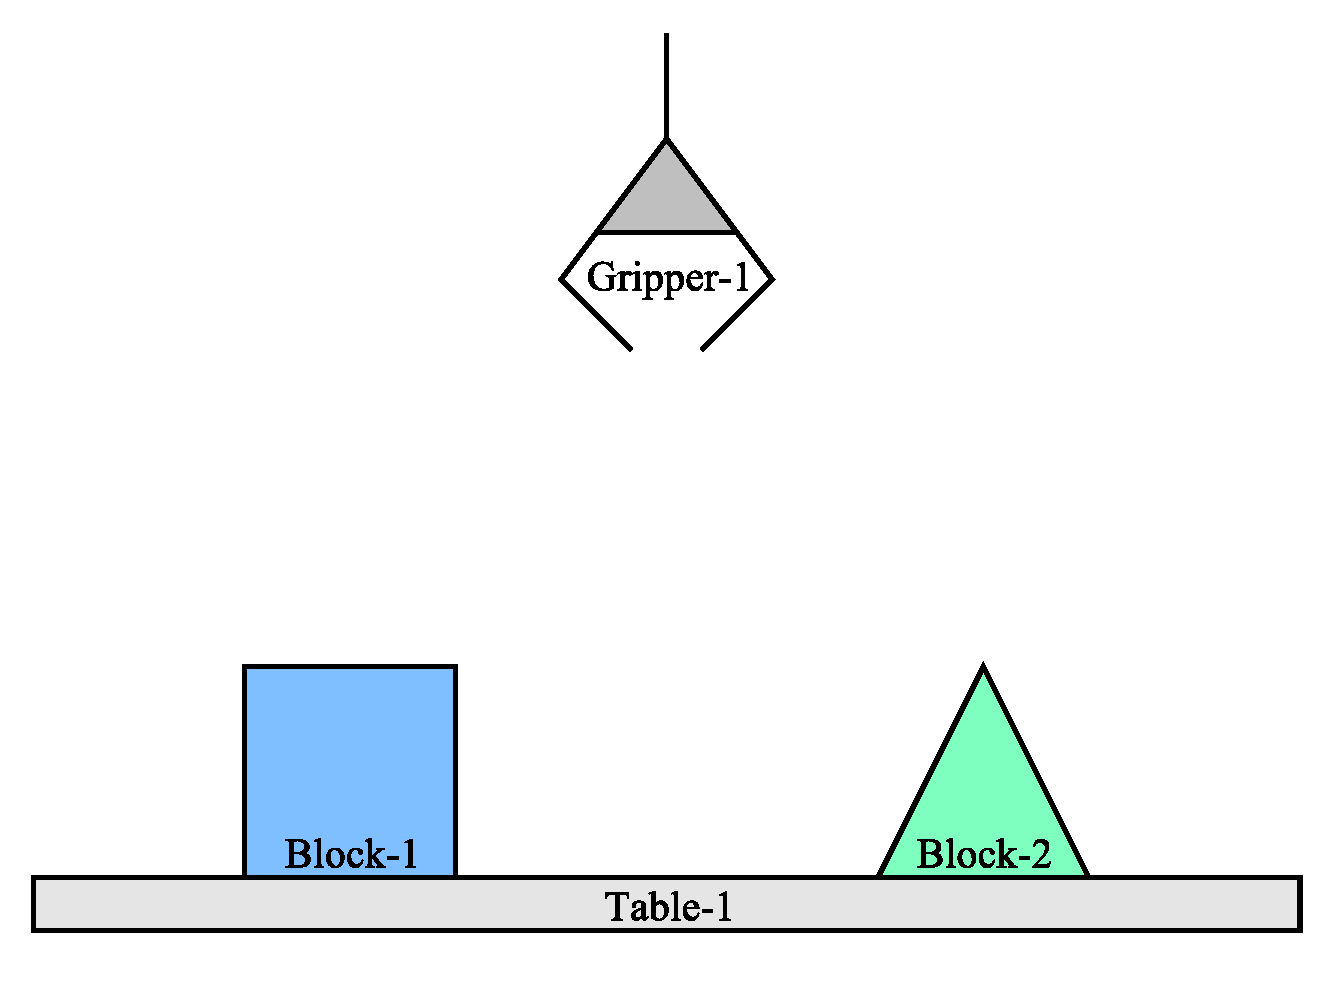
\includegraphics[width=10cm]{gfx/blocks_world_simulation}
\caption{An example for simulation.}
\label{figure:blocks_world_simulation}
\end{figure}

I will begin with one of the simplest mathematical models, a
\emph{set} of symbols, to model of the activities in Duration.  I will
first describe the simulation model as the mathematical set, X, the
activities of the state.  Here is an example of a possible
symbolization of the activities shown in
{\mbox{\autoref{figure:blocks_world_simulation}}}:
\begin{equation}
\label{equation:example_initial_state}
X =
  \left\{
    \begin{array}{l}
      \text{{\tt{Gripper-1}}}, \\
      \text{{\tt{Block-1}}}, \\
      \text{{\tt{Block-2}}}, \\
      \text{{\tt{Table-1}}} \\
      \text{{\tt{sitting-on}}}, \\
      \text{{\tt{being-above}}}, \\
      \text{{\tt{moving}}}, \\
      \text{{\tt{left}}}
    \end{array}
  \right\}
\end{equation}

\section{A Graph Representation}

The activities in Duration exist in a continuous Spatial arrangement
that is symbolized and ordered by the reflective thinking layers.  In
order to simulate this continuous homogenous Space, a discrete static
representation must be included in the state of the simulation model.
A graph of labelled nodes and edges can be used to represent the
activity of a Spatial relationship in the simulation.  Because the
graph provides a clear notation for referring to types of Spatial
arrangements of activities, a modified notation originally from
{\mbox{\cite{messmer:1995}}} is used to define a labelled graph in
{\mbox{Definition~\ref{definition:graph_first}}} and a labelled
subgraph in {\mbox{Definition~\ref{definition:graph_last}}}.

\begin{definition}
\label{definition:graph_first}
\emph{
A graph $G$ is the 4-tuple $(V, ~E, ~\mu, ~\nu)$, where
\begin{itemize}
\item $V$ is the set of vertices,
\item $E ~{\subseteq}~ V ~{\times}~ V$ is the set of edges,
\item $\mu : V \mapsto \{\ell_V\}$ is a function assigning a set of labels to each vertex.
\item $\nu : E \mapsto \{\ell_E\}$ is a function assigning a set of labels to each edge.
\end{itemize}
}\end{definition} \noindent In this definition, the edges are
directed, i.e. there is an edge from $v_1$ to $v_2$ if $(v_1,
v_2){\in}E$.  The empty graph, i.e. the graph with an empty set of
vertices will be denoted by $\emptyset$.  The union of the set of
labels referred to by $\mu$ and $\nu$ will be sometimes be referred to
with a dot notation, $\mathring{G}=\ell_V {\cup} \ell_E$.

\begin{definition}
\label{definition:graph_last}
\emph{ Given a graph $G = (V, E, \mu, \nu)$, a \emph{subgraph} of $G$
  is a graph $G_s = (V_s, E_s, \mu_s, \nu_s)$ such that
\begin{enumerate}
\item $V_s ~{\subseteq}~ V$
\item $E_s ~{\subseteq}~ V_s {\times} V_s$,
\item $\mu_s$ is the restriction of $\mu$, i.e.
\begin{align*}
\mu_s(e) &\subseteq
   {\left\{
      \begin{array}{ll}
        \mu(v)           & \text{if }v {\in} V_s \\
        \text{undefined} & \text{otherwise}
      \end{array}
    \right.}
\end{align*}
\item $\nu_s$ is the restriction of $\nu$, i.e.
\begin{align*}
\nu_s(e) &\subseteq
   {\left\{
      \begin{array}{ll}
        \nu(e)     & \text{if }e {\in} E_s \\
        \text{undefined} & \text{otherwise}
      \end{array}
    \right.}
\end{align*}
\end{enumerate}
}\end{definition} \noindent From this definition it is easy to see
that, given a graph $G$, any subset of its vertices and an included
subset of its edges uniquely defines a subgraph of $G$.  The notation
$G_s ~{\subseteq}~ G$ is used to indicate that $G_s$ is a subgraph of
$G$.

\section{Graph Isomorphism}

\begin{definition}
\label{definition:graph_isomorphism}
{\emph{A bijective function $f : V \mapsto V^\prime$ is a \emph{graph
      isomorphism} from a graph $G = \{V, E, \mu, \nu\}$ to a graph
    $G^\prime = \{V^\prime, E^\prime, \mu^\prime, \nu^\prime\}$ if:
\begin{enumerate}
\item $\mu(v) = \mu^\prime(f(v))$ for all $v \in V$.
\item For any edge $e\ =\ (v_1,\ v_2)\ \in\ E$ there exists an edge
  $e^\prime\ =\ (f(v_1),\ f(v_2))\ \in\ E^\prime$ such that
  $\nu(e)\ =\ \nu^\prime(e^\prime)$, and for any
  $e^\prime\ =\ (v^\prime_1,\ v^\prime_2)\ \in\ E^\prime$ there exists
  an edge $e\ =\ (f^{-1}(v^\prime_1),\ f^{-1}(v^\prime_2))\ \in\ E$
  such that $\nu^\prime(e^\prime)\ =\ \nu(e)$.
\end{enumerate}
}}\end{definition}

\section{Representing Continuous Space as a Graph}

{\mbox{\autoref{figure:simulation_example_state}}} shows an example of
the simulation state state represented as a graph.  Graph notation
will be used to describe the activities in Duration and continuous
Space, which exist before they are symbolized and discretely ordered
by the $\text{reflective}^1$ layer.  The simulation model state space,
$S$, is defined to be a graph in
{\mbox{Equations~\ref{equation:define_graph_state_first}}}
{\mbox{through~\ref{equation:define_graph_state_last}}}.
\begin{align}
\label{equation:define_graph_state_first}
       S &= (S_V, ~S_E, ~S_\mu, ~S_\nu) \\
     S_V &= \{v_1, ~v_2, ~v_3, ~v_4, ~v_5, ~v_6, ~v_7, ~v_8, ~v_9\} \\
     S_V &= {\left\{
               \begin{array}{l}
                 \text{\tt{Gripper}}, ~\text{\tt{Block}}, ~\text{\tt{Table}}, \\
                 \text{\tt{gripper-1}}, ~\text{\tt{block-1}}, ~\text{\tt{gripper-1}}, \\
                 \text{\tt{table-1}}, ~\text{\tt{left}}
               \end{array}
             \right\}} \\
     S_E &= {\left\{
               \begin{array}{l}
                 (v_1, v_5), ~(v_1, v_4), ~(v_1, v_9), ~(v_2, v_4), \\
                 (v_2, v_6), ~(v_3, v_4), ~(v_3, v_7), ~(v_4, v_8)
               \end{array}
             \right\}} \\
S_\mu(v) &=
  {\left\{
     \begin{array}{ll}
       \{\text{\tt{Gripper}}\}   & \text{if }v = v_1 \\
       \{\text{\tt{Block}}\}     & \text{if }v = v_2 ~{\vee}~ \\
                                 & \text{~ } v = v_3 \\
       \{\text{\tt{Table}}\}     & \text{if }v = v_4 \\
       \{\text{\tt{gripper-1}}\} & \text{if }v = v_5 \\
       \{\text{\tt{block-1}}\}   & \text{if }v = v_6 \\
       \{\text{\tt{block-2}}\}   & \text{if }v = v_7 \\
       \{\text{\tt{table-1}}\}   & \text{if }v = v_8 \\
       \{\text{\tt{left}}\}      & \text{if }v = v_9 \\
       \text{undefined}          & \text{otherwise}
     \end{array}
   \right.} \\
\label{equation:define_graph_state_last}
S_\nu(e) &=
  {\left\{
     \begin{array}{ll}
       \{\text{\tt{name}}\}        & \text{if }e = (v_1, v_5) ~{\vee}~ \\
                                   & \text{if }e = (v_2, v_6) ~{\vee}~ \\
                                   & \text{if }e = (v_3, v_7) ~{\vee}~ \\
                                   & \text{~ } e = (v_4, v_8) \\
       \{\text{\tt{being-above}}\} & \text{if }e = (v_1, v_4) \\
       \{\text{\tt{moving}}\}      & \text{if }e = (v_1, v_9) \\
       \{\text{\tt{sitting-on}}\}  & \text{if }e = (v_2, v_4) ~{\vee}~ \\
                                   & \text{~ } e = (v_3, v_4) \\
       \text{undefined}            & \text{otherwise}
     \end{array}
   \right.}
\end{align}
\begin{figure}
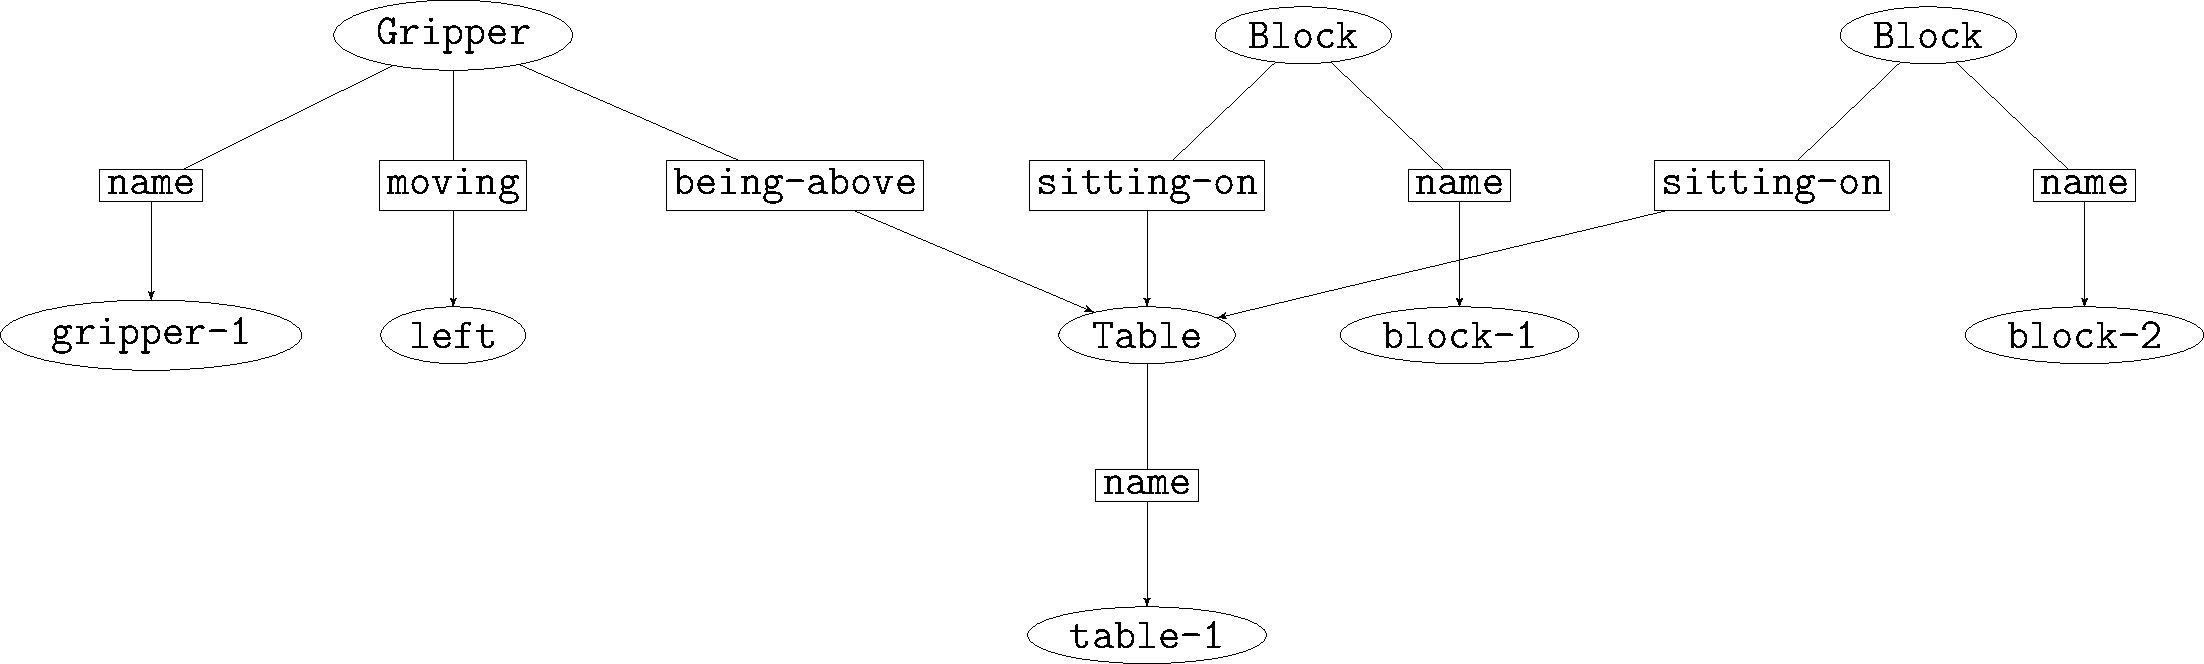
\includegraphics[width=12cm]{gfx/simulation_example_state}
\caption[A labelled graph representation of a state space.]{A labelled
  graph representation of a state space, where circles represent
  nodes, and squares represent edges.}
\label{figure:simulation_example_state}
\end{figure}

\section{Dot Notation for Graph-based Frame Objects}

Sometimes it is useful to refer to parts of a graph by considering
nodes in the graph to represent frame objects that have slotted
relationships with other frame objects.  Thus, I use a dot notation to
refer to the set of nodes that are connected to a given node, $v_1$,
through a given edge label, $\ell_e$, as defined in
{\mbox{\autoref{equation:frame_dot_notation}}}.
\begin{equation}
\label{equation:frame_dot_notation}
v_1.\ell_e = \{v_2 ~:~ (v_1, v_2) \in S_E \wedge \ell_e \in \nu[(v_1, v_2)]\}
\end{equation}

\section{Simulated Existence}

Activities in continuous Space actually exist.  Once we have
considered the activities in Duration to be the set of symbols, $S$,
we have assumed static representations for the actual dynamic.  The
dynamic does not have terms to help us in representing.  Therefore,
the question of existence becomes a question of whether or not a
symbol is in the set that is the current state of the simulation, $S$.
Equation~\ref{equation:define_exists} shows a definition of {\tt
  exists}, defined as the subgraph relationship between any state,
$G$, represented as a labelled graph, and the currently simulated
state graph, $S$:
\begin{equation}
\label{equation:define_exists}
\text{exists}(G) \longleftrightarrow G ~{\subseteq}~ S
\end{equation}




% Original definition of a graph as a 4-tuple with labelled nodes and edges

%\begin{definition}
%\label{definition:graph_first}
%\emph{
%A graph $G$ is the 4-tuple $(V, ~E, ~\nu, ~\nu)$, where
%\begin{itemize}
%\item $V$ is the set of vertices,
%\item $E ~{\subseteq}~ V ~{\times}~ V$ is the set of edges,
%\item $\nu : V \mapsto \ell_V$ is a function assigning a label to each vertex,
%\item $\nu : E \mapsto \{\ell_E\}$ is a function assigning a set of labels to each edge.
%\end{itemize}
%}\end{definition} \noindent In this definition, the edges are
%directed, i.e. there is an edge from $v_1$ to $v_2$ if $(v_1,
%v_2){\in}E$.  The empty graph, i.e. the graph with an empty set of
%vertices will be denoted by $\emptyset$.  The union of the sets of
%labels referred to by $\nu$ and $\nu$ will be sometimes be referred to
%with a dot notation, $\mathring{G}=\ell_V {\cup} \ell_E$.
%
%\begin{definition}
%\label{definition:graph_last}
%\emph{ Given a graph $G = (V, e, \nu, \nu)$, a \emph{subgraph} of $G$
%  is a graph $G_s = (V_s, e_s, \nu_s, \nu_s)$ such that
%\begin{enumerate}
%\item $V_s ~{\subseteq}~ V$
%\item $E_s ~{\subseteq}~ V_s {\times} V_s$,
%\item $\nu_s$ and $\nu_s$ are the restrictions of $\nu$ and $\nu$,
%  respectively, i.e.
%\begin{align*}
%\nu_s(v) &=         {\left\{
%                       \begin{array}{ll}
%                         \nu(v)           & \text{if }v {\in} V_s \\
%                         \text{undefined} & \text{otherwise}
%                       \end{array}
%                     \right.} \\
%\nu_s(e) &\subseteq {\left\{
%                       \begin{array}{ll}
%                        \nu(e)           & \text{if }e {\in} E_s \\
%                        \text{undefined} & \text{otherwise}
%                       \end{array}
%                     \right.}
%\end{align*}
%\end{enumerate}
%}\end{definition}



%\section{Simulating the Plan}
%


%\section{State Transitions (should be rewritten in simulation objects)} 

%\autoref{figure:blocks_world_gripper_over_block} shows an example of
%the next state of the simulation, $S[1]$.
%Equation~\ref{equation:example_next_state} gives an example
%description of the next state of the simulation model:
%\begin{figure}[bth]
%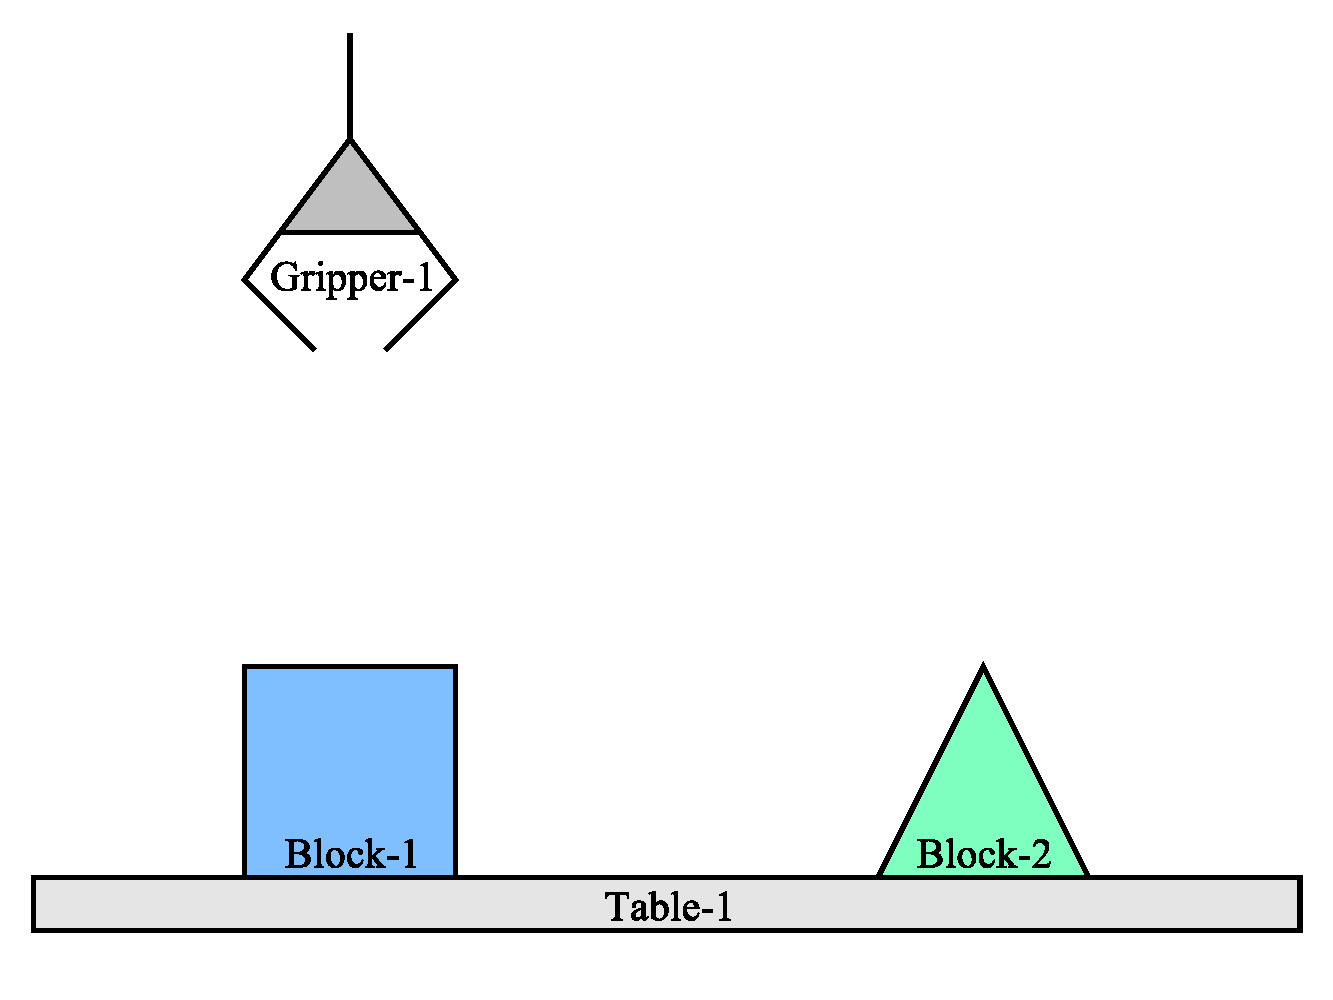
\includegraphics[width=10cm]{gfx/blocks_world_gripper_over_block}
%\caption{An example future state of simulation.}
%\label{figure:blocks_world_gripper_over_block}
%\end{figure}
%\begin{equation}
%\label{equation:example_next_state}
%S[1] =
%  \left\{
%    \begin{array}{l}
%      \text{{\tt Block-1-sitting-on-Table-1}}, \\
%      \text{{\tt Block-2-sitting-on-Table-1}}, \\
%      \text{{\tt Gripper-1-hovering-above-Table-1}}, \\
%      \text{{\tt Gripper-1-hovering-above-Block-1}}
%    \end{array}
%  \right\}
%\end{equation}
%
%Now, in order to begin to describe the activity of simulation, we must
%explicitly represent the transition, $T$, from one state to another.
%I refer to the resulting change to the state of the simulation as a
%\emph{state transition}.  The transition, $T[n]$, consists of two sets
%that keep track of changes, the \emph{add} set and the \emph{remove}
%set, as shown in Equation~\ref{equation:state_transition}:
%\begin{equation}
%\label{equation:state_transition}
%T[n] = \{T_\text{add}[n], ~T_\text{remove}[n]\}
%\end{equation}
%Equations~\ref{equation:predictive_state_transition}
%through~\ref{equation:transframe_last} give a definition of the
%transition, $T[n]$, in terms of the states, $S[n]$ and
%$S[n+1]$:
%\begin{align}
%\label{equation:predictive_state_transition}
%          S[n+1] & = S[n] ~{\cup}~ T_\text{add}[n] ~{\setminus}~ T_\text{remove}[n] \\
%         T_\text{remove}[n] & ~{\subseteq}~ S[n] \\
%         T_\text{remove}[n] & ~{\not\subseteq}~ S[n+1] \\
%            T_\text{add}[n] & ~{\subseteq}~ S[n+1] \\
%\label{equation:transframe_last}
%            T_\text{add}[n] & ~{\not\subseteq}~ S[n]
%\end{align}
%Equations~\ref{equation:state_transition_first}
%and~\ref{equation:state_transition_last} give the state transition,
%$T[n]$, for every step of the simulation:
%\begin{align}
%  \label{equation:state_transition_first}
%     T_\text{add}[n] &= S[n+1] ~{\setminus}~ S[n] \\
%  \label{equation:state_transition_last}
%  T_\text{remove}[n] &= S[n]   ~{\setminus}~ S[n+1]
%\end{align}
%Equation~\ref{equation:predictive_state_transition} shows the
%predictive potential for knowing the transition, $T[n]$, given the
%current state, $S[n]$.  Of course, $T[n]$ is defined in
%terms of $S[n]$ \emph{and} $S[n+1]$, so any
%predictive potential for
%Equation~\ref{equation:predictive_state_transition} is purely
%hypothetical.

